\chapter{Introduction}
%\section{Introduction}
\label{ch:1}
The term "knowledge graph" gained popularity in 2012 when Google launched its own "\textit{Google Knowledge Graph}". A knowledge graph is a collection of data represented as a graph. There are many ways of modelling using graphs. The most commonly used ones are directed edge-labelled graphs, heterogeneous graphs, property graphs and graph dataset \cite{Hogan2021}. In this report, we consider directed edge-labelled graphs for modelling knowledge graphs.

A directed edge-labelled graph, also known as a multi-relational graph, consists of a set of nodes and a set of directed labelled edges \cite{Hogan2021}. Information represented in knowledge graphs conveys knowledge of the real world, where the nodes represent entities of interest and the directed edges represent the many different binary relations between those entities. Entities are real world objects and abstract concepts. An object is a physical item in the real world such as a university (e.g., Technical University Dresden) or a planet (e.g., Earth). A concept on the other hand, refers to general categories of objects such as chemical element or philosopher. 

For example, the information
 \begin{verbatim}
 	\texttt{"Helium is a type of chemical element that has the chemical formula He"}
	\end{verbatim}
can be represented using a directed edge-labelled graph. The nodes of the graph would represent the entities "\texttt{Helium}", "\texttt{chemical element}" and "\texttt{He}". There would be two labelled edges, one pointing from the "\texttt{Helium}" node to the "\texttt{chemical element}" node, and the other from the "\texttt{Helium}" node to the "\texttt{He}" node. These edges would represent the relations "\texttt{instance of}" and "\texttt{chemical formula}" respectively. Figure~\ref{fig:1} shows such a directed-edge labelled graph. We provide a more complex example later in Chapter~\ref{ch:2}.

\begin{figure}[b!tp]
  \centering
  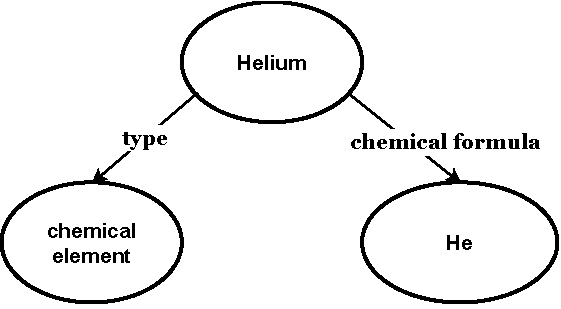
\includegraphics[width=0.75 \linewidth]{images/knowledge_graph.drawio.pdf}
  \caption{A directed-edge labelled graph}
  \label{fig:1}
\end{figure}

Resource Description Framework (RDF) \cite{R.Cyganiak2014} is a standard framework that models the Semantic Web. Its data model is based on directed edge-labelled graphs and is composed of a set of triples or statements. Each triple consist of a subject node, predicate edge and an object node. The subject and object nodes represent the source and destination respectively while the predicate edge connects these two nodes, representing a binary relationship between them. RDF is useful for describing and exchanging graphs over the web. 

Knowledge graphs have practical uses in commercial and scientific domains. Many companies such as Amazon, Facebook, Uber and Google use knowledge graphs for their applications. For example, Google and Bing use their knowledge graphs, Google Knowledge Graph and Satori respectively, to enhance the results in their search engines. In the field of life sciences, various knowledge graphs such as Neurocommons and LinkedLifeData exist that contain biomedical information from different sources \cite{Nickel2015}. 

Depending on the organization or community there are open or enterprise knowledge graphs \cite{Hogan2021}. Open knowledge graphs include Wikidata, DBpedia, Freebase and YAGO. These are available online and freely accessible to the public. On the other hand, enterprise knowledge graphs are used internally within companies and are aimed towards solving their specific use-cases

We focus on Wikidata in this report. Wikidata \cite{Foundationa} is a free and publicly available knowledge base that can be read and edited by both humans and machines. It is one of the many projects by Wikimedia Foundations such as Wikipedia, Wikibooks, Wikimedia Commons and Wikitionary. Wikidata was created in 2012 at Wikimedia Deutschland by a community of volunteers. These volunteers edit and control all content. As of December 2022, Wikidata has more 23000 active editors.\footnote{https://wikidata.wikiscan.org/}

One of the original purposes behind the creation of Wikidata was to help its sister projects. Initially, Wikipedia and its sister projects maintained their own lists of interlanguage links. These refer to links between Wikipedia articles about the same topic in different languages. The interlanguage links were provisioned via Wikidata after 2012. Wikidata is also used to display data shown inside Wikipedia pages. The usage of this mainly depends on the language of the Wiki. For instance, in the case of some languages, parts of the Wikipedia pages are automatically created from the data in Wikidata. Others, especially those of less common languages that are not widely used, use Wikidata to create placeholder pages when an article may not be in their respective language. In 2018, around 59\% of Wikidata information was used in English Wikipedia articles, although mostly for external identifiers and coordinate locations \cite{Wikipedia2017}. 

Wikidata stores information in the form of structured data in a database \cite{Tharani2021}. This is not the case for its sister projects as they contain unstructured data. The information on their web pages is not directly given a structure in the form of tables or lists. Wikidata acts as a central storage for these projects and focuses on providing a structure for their data \cite{Wikidata2014}. Additionally, Wikidata also supports linked data. This means that the data stored can be linked to datasets and databases like Google Books and OmegaWiki. Wikidata can also be used for quality checks against Wikipedia articles. This is useful when information about a specific topic needs to be known and the solution is easily found by querying the knowledge graph, in this case Wikidata.

Moreover, there is also a wide range of commercial and research oriented applications for Wikidata. This is due to the fact that it has a large amount of real world data. For instance, Wikidata has external usages in many large organizations such as Eurowings, Google, Apple and Amazon. This includes tasks such as data integration, authority control, identity providing and data-driven journalism. In the field of research, Wikidata is used for collecting test data for knowledge graph related algorithms and training data for machine learning projects.

SPARQL \cite{C.B.Aranda2013} is a W3C standard query language based on matching graph patterns. It is used to query information from any source that maps its data in RDF format. Wikidata is built on RDF framework and can be can be queried using SPARQL. SPARQL has gained widespread popularity in research and academics. However, in commercial applications like application development, SPARQL faces some potential barriers. This is mainly due to the complex nature of SPARQL queries, and the lack of libraries and frameworks to facilitate its integration in applications. 

GraphQL \cite{GraphQLa} is an open source query language popular in commercial applications. It was developed by Facebook in 2012 and was made open source later in 2015. It is easy to learn and use, providing syntax that is more human friendly than SPARQL. It is possible to implement GraphQL in different programming languages and many libraries exist to support the integration into application development. Queries in GraphQL have a tree-like structure, where the root or parent node is the object and the children nodes are the fields for that object. The obtained results have the same shape as the queries, and this implies that we always get back what we expect. In other words, the users decide which information to obtain from the server by GraphQL APIs. This makes GraphQL convenient to use as opposed REST APIs, where the decision is made by the server. 

Owing to the simplistic nature of GraphQL queries and its ease of integration in application development, GraphQL is a prospective approach to query RDF data. Consequently, this further opens the scope of using knowledge graphs for querying and having a better understanding of the data that lies within them.

In this report, we research on existing mechanisms to query RDF data using GraphQL. We mainly focus on two approaches - GraphQL-LD and HyperGraphQL. Both of these are open source and can be used to query arbitrary knowledge graphs using GraphQL. We show how these two approaches can be used to query Wikidata. We also show how these two compare with each other in terms of usage as well as their ability to express important features that are available in standard GraphQL specifications and SPARQL.


The remainder of the report is structured as follows.
\begin{itemize}
	\item In Chapter~\ref{ch:2}, we provide an overview of RDF, Wikidata, SPARQL and GraphQL. We also show some important differences between GraphQL and SPARQL. 
	\item In Chapter~\ref{ch:3}, we show the existing approaches used to query RDF graphs using GraphQL, focusing on GraphQL-LD and HyperGraphQL.
	\item In Chapter~\ref{ch:4}, we provide implementation of GraphQL-LD and HyperGraphQL to query actual data from Wikidata.
	\item In Chapter~\ref{ch:5}, we compare GraphQL-LD and HyperGraphQL in terms of their implementation. We also show comparison based on important features that are available in standard GraphQL specifications and SPARQL.
\end{itemize}